\documentclass[letterpaper,12pt,fleqn]{article}
\usepackage{matharticle}
\pagestyle{empty}
\newcommand{\norm}[1]{\left\lVert#1\right\rVert}
\newcommand{\nc}{\norm{\cdot}}
\newcommand{\bn}{B_{\nc}}
\newcommand{\vx}{\vec{x}}
\renewcommand{\a}{\alpha}
\renewcommand{\b}{\beta}
\begin{document}
\section*{Unit Ball of a Vector Norm}

\begin{definition}[Unit Ball]
  Let $\nc$ be a vector norm on $\C^n$. The \emph{closed unit ball} of $\nc$,
  denoted $\bn$, is given by:
  \[\bn=\{\vx\in\C^n\mid\norm{\vx}\le1\}\]
\end{definition}

Note that when $n=1$:

\begin{minipage}{3.5in}
\begin{itemize}
\item $\ell_1,\ell_2,\ell_{\infty}$ are the same.
\item $B_{\ell_1}=B_{\ell_2}=B_{\ell_{\infty}}=\{z\in\C\mid\abs{z}\le1\}$
\end{itemize}
\end{minipage}
\begin{minipage}{3in}
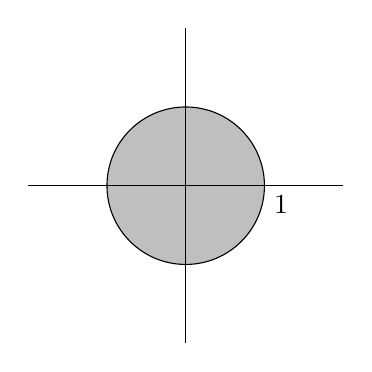
\begin{tikzpicture}
  \draw [fill=lightgray] (0,0) circle [radius=1];
  \node [below right] at (1,0) {$1$};
  \draw (-2,0) -- (2,0);
  \draw (0,-2) -- (0,2);
\end{tikzpicture}
\end{minipage}

If restricted to $\R^2$ then we have the following:

\newcommand{\xy}{\begin{bmatrix} x \\ y \end{bmatrix}}

\begin{minipage}{3in}
  $B_{\ell_1}=\left\{\xy\mid\abs{x}+\abs{y}\le1\right\}$
\end{minipage}
\begin{minipage}{3in}
  \begin{tikzpicture}
    \draw (-2,0) -- (2,0);
    \draw (0,-2) -- (0,2);
    \node [below right] at (1,0) {$1$};
    \draw (1,0) -- (0,1) -- (-1,0) -- (0,-1) -- cycle;
  \end{tikzpicture}
\end{minipage}

\begin{minipage}{3in}
  $B_{\ell_2}=\left\{\xy\mid\sqrt{x^2+y^2}\le1\right\}$
\end{minipage}
\begin{minipage}{3in}
  \begin{tikzpicture}
    \draw (-2,0) -- (2,0);
    \draw (0,-2) -- (0,2);
    \node [below right] at (1,0) {$1$};
    \draw (0,0) circle [radius=1];
  \end{tikzpicture}
\end{minipage}

\begin{minipage}{3in}
  $B_{\ell_{\infty}}=\left\{\xy\mid\max\{x,y\}\le1\right\}$
\end{minipage}
\begin{minipage}{3in}
  \begin{tikzpicture}
    \draw (-2,0) -- (2,0);
    \draw (0,-2) -- (0,2);
    \node [below right] at (1,0) {$1$};
    \draw (-1,-1) rectangle (1,1);
  \end{tikzpicture}
\end{minipage}

Note that $\forall\,\vx$ we have:
\[\norm{\vx}_{\infty}\le\norm{\vx}_2\le\norm{\vx}_1\]
However:
\[B_{\ell_1}\subseteq B_{\ell_2}\subseteq B_{\ell_{\infty}}\]

\begin{theorem}
  $\forall\vx\in\C^n$:
  \[\norm{\vx}_{\a}\le\norm{\vx}_{\b}\iff B_{\nc_{\a}}\supseteq B_{\nc_{\a}}\]
  The larger the norm, the smaller the unit ball.
\end{theorem}

\end{document}
